\documentclass[serbian]{article}

\usepackage{amsmath}
\usepackage{float}
% \usepackage{floatrow}
\usepackage[T1, T2A]{fontenc}
\usepackage[serbian]{babel}
\usepackage[utf8]{inputenc}
\usepackage{xcolor}
\usepackage{fancyhdr}

\usepackage[a4paper, total={6in, 8in}]{geometry}
\usepackage{graphicx}
\usepackage[colorlinks=true, allcolors=blue]{hyperref}
\usepackage{hyperref}

\usepackage{pgfplots}
\pgfplotsset{width=10cm,compat=1.9}

% We will externalize the figures
\usepgfplotslibrary{external}
\tikzexternalize

\hypersetup{colorlinks,linkcolor={blue},citecolor={blue},urlcolor={blue}}  

\title{\textbf{KONSTRUKCIJA I ANALIZA ALGORITAMA II} \\
\vspace{25}
\Large{\textbf{Algoritmi za konstrukciju sufiksnog niza linearne složenosti}}}
\author{ \\\\Miloš Milaković, 1052/2021 \\ \textit{mi211052@alas.matf.bg.ac.rs} \\\\\\
        \textit{profesor:} dr Vesna Marinković \\
        \textit{asistent:} Jelena Marković \\\\\\}

\date{Beograd 2024.}

\begin{document}

\maketitle
\thispagestyle{empty} 

\vspace{17}
\begin{figure}[h!]
    \centering
    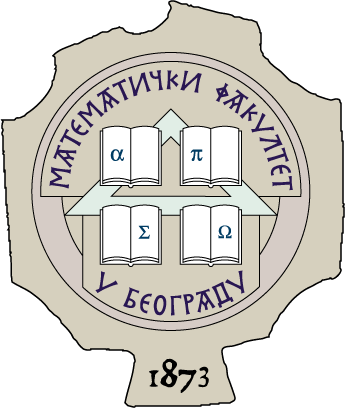
\includegraphics[width=4cm, height=4cm]{grb.png}
\end{figure} 

\newpage
\tableofcontents

\newpage
\section{Uvod}
\textbf{Sufiksni niz} predstavlja strukturu podataka koja može na efikasan način da reši određene probleme koje se javljaju u oblasti informatike, poput problema pronalaženja određene reči u tekstu, traženje palindroma u tekstu, upoređivanje niski, poravnanje genoma u bioinformatici. Dugi niz godina, sufiksni niz je bila inferiornija struktura podataka u odnosu na sufiksno stablo jer nije postojao efikasan algoritam, u linearnoj složenosti, za konstrukciju ove strukture a da taj algoritam nije koristio sufiksna stabla. Ova situacija se menja 2003. godine kada se pojavljuje više algoritama koji u linearnoj složenosti mogu da konstruišu sufiksni niz bez upotrebe sufiksnih stabala. Sufiksni nizovi postaju struktura koja se sve više koristi i koja dobija prednost u odnosu na sufiksna stabla pre svega zbog manjeg korišćenja memorije.\\

U ovom radu, biće predstavljen algoritam \textit{\textbf{DC3}}, kao i algoritam \textit{\textbf{SA-IS}}, sa određenim primerima, rezultatima i kodom koji realizuje ove algoritme.

\section{Definicije i pojmovi}
\textbf{Definicija:} \textbf{Sufiksni niz} niske \textit{S} je niz celih brojeva koji predstavljaju početne pozicije (indekse) sufiksa niske S koji su leksikografski sortirani.\\

\textbf{Primer:} Posmatrajmo nisku \textit{S = abcabcacab}. Ovo je niska od 10 karaktera a sufiksni niz \textit{SA} koji je određen ovom niskom je:

\begin{equation}
\mathbf{SA = \{8, 0, 3, 6, 9, 1, 4, 7, 2, 5\}}
\end{equation}

U tabeli \ref{table:1} mogu da se vide svi sufiksi niske \textit{S} leksikografski sortirani.

\begin{table}[h!]
    \begin{center}
        \begin{tabular}{|l|l|} \hline
        \textbf{Indeks niske S} & \textbf{Sufiks}\\ \hline
        8 & ab\\ \hline
        0 & abcabcacab\\ \hline
        3 & abcacab\\ \hline
        6 & acab\\ \hline
        9 & b\\ \hline
        1 & bcabcacab\\ \hline
        4 & bcacab\\ \hline
        7 & cab\\ \hline
        2 & cabcacab\\ \hline
        5 & cacab\\ \hline
        \end{tabular}
        \caption{Tabela sufiksa niske \textit{S} leksikografski sortirani i njihovih indeksa}
        \label{table:1}
    \end{center}
\end{table}

\textbf{Definicija:} \textbf{Rang} elementa x u nizu S je broj elemenata u nizu S koji su manji od elementa x. U slučaju sufiksnog niza, to predstavlja poziciju na kojoj se zadati element nalazi u sufiksnom nizu.

\section{Algoritam DC3}

\textbf{DC3} algoritam je rekurzivni algoritam koji u linearnom vremenu konstruiše sufiksni niz \cite{sanders_peter, presentation_dc3, master_dc3}. Algoritam koristi \textit{radix} sortiranje kao efikasnu tehniku za poređenje niski. Ulazna niska je konvertovana u niz brojeva tako što se svaki karakter pretvori u broj i samim tim je olakšana primena \textit{radix} sorta. Ovaj algoritam deli sufikse u dve grupe i sortira svaku grupu posebno. Time što su sufiksi podeljeni u dve grupe, algoritam koristi jednu grupu da sortira drugu grupu i izbegava ponavljanje poređenja. Na kraju, ove dve grupe se spajaju i konstruiše se sufiksni niz.

U situacijama kada u konvertovanoj nisci, počevši od nekog indeksa koji je deljiv sa 1 ili 2, ne možemo da napravimo sekvencu od 3 broja nego nam fali još brojeva, konvertovana niska se dopunjuje onolikim brojem nula koliko nam je potrebno da bi mogle da se naprave trojke uzoraka.

 \subsection{Korak 0: Konvertovanje karaktera niske u brojeve}
Od ulazne niske kreira se niz brojeva tako što se svaki karakter ulazne niske pretvara u broj i na kraj doda doda tri nule. Dodate nule će se iskoristiti za konstrukciju trojki uzoraka u sledećem koraku.

\subsection{Korak 1: Sortiranje uzoraka sufiksa}
Konstruiše se sufiksni niz za sufikse koji počinju na pozicijama \textit{i}, takvim da je ostatak prilikom deljenja pozicije \textit{i} sa 3 različit od 0. U ovom koraku svaki sufiks u sufiksnom nizu je dužine 3 počevši od pozicije \textit{i}.

\begin{table}[h!]
    \begin{center}
        \begin{tabular}{|c|c|c|c|c|c|c|c|c|c|c|c|c|} \hline
        97 & 98 & 99 & 97 & 98 & 99 & 97 & 99 & 97 & 98 & 0 & 0 & 0\\ \hline
        0 & 1 & 2 & 3 & 4 & 5 & 6 & 7 & 8 & 9 & 10 & 11 & 12\\ \hline
        \end{tabular}
        \caption{Konvertovana niska \textit{abcabcacab} sa indeksima}
        \label{table:2}
    \end{center}
\end{table}

Posmatrajući tabelu \ref{table:2} dobijamo da sledeći indeksi prilikom deljenja sa 3 daju ostatak 1 ili 2, gde su prvo navedeni indeksi koji daju ostatak 1 prilikom deljenja:
\begin{equation}
\mathbf{SA_{12} = \{1, 4, 7, 10, 2, 5, 8\}}
\end{equation}

U ovom slučaju ne koriste se indeksi 11 i 12 jer počevši od njihove pozicije neće moći da se kreira sekvenca od 3 broja.

Nakon toga indekse u nizu \(SA_{12}\) konvertujemo u sekvence od 3 broja, tako da dobijamo sledeći niz:
\begin{equation}
\mathbf{SA_{12} = \{98, 99, 97\}, \{98, 99, 97\}, \{99, 97, 98\} , \{0, 0, 0\} , \{99, 97, 98\} , \{99, 97, 99\} , \{97, 98, 0\} }
\end{equation}

Sada se primenjuje radiks sortiranje, porede se prvi članovi svih trojki. Dobijamo sledeći rezultat:
\begin{equation}
\mathbf{SA_{12} =  \{0, 0, 0\}, \{97, 98, 0\} ,\{98, 99, 97\}, \{98, 99, 97\}, \{99, 97, 98\} , \{99, 97, 98\} , \{99, 97, 99\} }
\end{equation}

Radiks sortiranje se mora primeniti više puta jer među nekim trojkama su isti prvi članovi i samim tim nismo skroz sigurni koji je pravi redosled tih trojki. Prave se grupe gde je isti prvi član pa se te grupe posebno sortiraju po drugom članu trojke.
\begin{equation}
\mathbf{G1 = \{98, 99, 97\}, \{98, 99, 97\}}
\end{equation}
\begin{equation}
\mathbf{G2 = \{99, 97, 98\} , \{99, 97, 98\} , \{99, 97, 99\}}
\end{equation}

Drugi članovi grupe \textit{G1} kao i drugi članovi grupe \textit{G2} su isti, tako da se te 2 grupe sortiraju i po trećem članu.

Konkretno u slučaju grupe \textit{G1} neće biti promena pošto su njeni članovi isti, ali će kod grupe \textit{G2} doći do promene pošto postoji različit treći član.\\\\


U slučaju da su svi elementi koje smo sortirali pomoću radiks sorta različiti nastavljamo dalje sa algoritmom. Ako postoje bilo koja 2 elementa koja su ista, onda ovaj algoritam pozivamo rekurzivno.\\\\

Krajnji rezultat ovog koraka je sortirani niz sufiksa koji počinju na indeksima koji nisu deljivi sa 3.

\subsection{Korak 2: Sortiranje sufiksa koje nismo do sada}
U ovom koraku sortiramo elemente čiji indeks prilikom deljenja sa 3 daje ostatak 0.
Kreiramo niz parova gde je prvi član vrednost iz konvertovanog početnog niza a drugi član je sam indeks.
Opet radimo radiks sort ali samo po prvom članu ovih parova. U slučaju da su svi prvi članovi različiti sufiksi će biti sortirani. Rezultat ovog koraka će biti niz koji sadrži druge članove ovih sortiranih parova, odnosno rezultat će biti sortirani niz indeksa na kojima počinju sufiksi.

Ako se desi da su neki prvi elementi ovih parova isti, moramo da iskoristimo već sortirani sufiksni niz sa indeksima čiji je ostatak 1 ili 2 pri deljenju sa 3. Na osnovu indeksa u parovima posmatramo koja je pozicija indeksa uvećanog za 1 u sortiranom nizu i koristimo tu vrednost kao prvi element parova koji će se dalje porediti. Ovo je ispravno zato što već imamo sortirane sufikse koji počinju na indeksima čiji je ostatak 1 ili 2 prilikom deljenje sa 3, a uvećavanjem indeksa koji je deljiv sa 3 za 1, dobićemo tačno indeks čiji je ostatak 1 pri deljenju sa 3, a njegovu poziciju već znamo.

Krajnji rezultat ovog koraka je sortirani niz indeksa koji su deljivi sa 3.

\subsection{Korak 3: Spajanje sortiranih nizova}
Poslednji korak ovog algoritma je da spojimo sortirane nizove.
Redom idemo kroz oba niza i koristeći sortirane indekse iz tih nizova poredimo vrednosti iz originalnog niza koji je konvertovan u brojeve - \textit{T}.
\begin{enumerate}
    \item Ako je \textit{T[i]} < \textit{T[j]} ili \textit{T[i]} > \textit{T[j]}, u zavisnosti od onoga što je manje, taj indeks će se dodati u sufiksni niz. Pokazivač u nizu iz kog je uzet indeks se uvećava za 1.
    \item Ako su ove dve vrednosti jednake poredimo vrednosti iz niza čiji su indeksi uvećani za 1. Ovde može da se iskoristi prednost toga što je već poznat sufiksni niz niza indeksa čiji su ostaci 1 i 2 prilikom deljenja sa 3. Ako je ostatak 1 prilikom deljenja pokazivača drugog niza sa 3, onda uvećevanjem za 1 dobijamo element koji i dalje pripada drugom nizu, a uvećavanjem pokazivača prvog niza za 1, njegov ostatak će biti 1, tako da dobijamo elemente koji pripadaju drugom nizu a sufiksni niz drugog niza već znamo. U slučaju da je ostatak 2 prilikom deljenja pokazivača drugog niza sa 3, onda uvećevanjem za 1 dobijamo element koji pripada prvom nizu, a uvećavanjem pokazivača prvog niza za 1, njegov ostatak će biti 1, i pripada drugom nizu. U ovom slučaju smo dobili elemente koji pripadaju različitim nizovima pa je njihovo poređenje potrebno.
\end{enumerate}

Kada prođemo kroz sve indekse jednog niza, elemente preostalog niza samo dodamo na kraj sufiksnog niza i dobićemo traženi rezultat.

\subsection{Složenost algoritma}

\textbf{Nulti korak} predstavlja pripremu niske i transformisanje u niz brojeva. Obuhvata jedan prolazak kroz niz tako da je njegova složenost \textit{O(n)}, gde je \textit{n} broj karaktera.

\textbf{Prvi korak} obuhvata pozicije koje daju ostatak 1 ili 2 prilikom deljenja sa 3. Broj takvih pozicija je \textit{2n/3}. Svaki od koraka zahteva linearno vreme tako da je složenost ovog koraka isto linearna.

\textbf{Drugi korak} obuhvata sortiranje sufiksa koje nismo do sada uz pomoć \textit{radix} sortiranja prvi elemenata parova koji ima \textit{n/3}. Uslučaju da ima istih elemenata potreban je još jedan prolazak kroz niz preostalih sufiksa da bi se odredili koji su sledeći indeksi koji se porede. Zbog prethodno navedenog složenost ovog koraka je \textit{O(n)}, gde je \textit{n} broj karaktera.

\textbf{Treći korak} predstavlja objedinjavanje dva sortirana dela niza tako što se prolazi kroz ta dva dela, pri čemu se ide do kraja jednog ili drugog kraja niza a ostatak elemenata se doda na kraj, tako da je složenost ovog koraka isto \textit{O(n)}, gde je \textit{n} broj karaktera.
\\\\
S obzirom da je složenost svakog od koraka \textit{O(n)}, može se zaključiti da će i ukupna složenost algoritma biti \textit{O(n)}, gde je \textit{n} broj karaktera.

Jedino u prvom koraku može da se desi da dođe do rekurzije i onda dobijamo rekurentnu jednačinu sledećeg tipa:+
\begin{equation}
\mathbf{T(n) = T(2n/3) + O(n)}
\end{equation}

Rešavanjem ove rekurentne jednačine dobija se da je složenost takođe \textit{O(n)}, gde je \textit{n} broj karaktera.

\section{Algoritam SA-IS}
Algoritam \textit{Suffix Array by Induced Sorting} na osnovu sortiranih delova sufiksnog niza pokušava da sortira i ostale delove sufiksnog niza koji već nisu sortirani \cite{sais, presentation_sais, master_sais}.

Ako imamo nisku \textit{S} na nju dodajemo karakter \textit{\$} koji predstavlja sentinel i služiće da predstavlja praznu nisku. \\\\

\textbf{Definicija:} \textbf{L-tip} u niski \textit{S} je svaki onaj karakter koji je veći od karaktera koji se nalazi na sledećoj poziciji.\\\\

\textbf{Definicija:} \textbf{S-tip} u niski \textit{S} je svaki onaj karakter koji je manji od karaktera koji se nalazi na sledećoj poziciji.\\\\

\textbf{Definicija:} \textbf{LMS pozicija} (\textit{leftmost S}) je svaki onaj karakter koji je S-tip u niski \textit{S} a koji se nalazi sa desne strane karaktera koji je L-tip.\\\\

\textbf{Definicija:} \textbf{LMS interval} predstavlja interval od jedne LMS pozicije do druge LMS pozicije pri čemu nema drugih LMS pozicija između njih. LMS interval određuje i LMS podnisku niske \textit{S}.\\\\

Algoritam se sastoji od narednih koraka:
\begin{enumerate}
    \item Generiši niz S/L tipova za nisku \textit{S}
    \item Nađi sve LMS pozicije
    \item Sortiraj sufikse na LMS pozicijama
    \item Sortiraj preostale sufikse
\end{enumerate}

\subsection{Korak 1: Generiši niz S/L tipova za nisku}
Prolaskom kroz nisku, s desna na levo, možemo da generišemo niz S/L tipova. Karakter na poslednjoj poziciji je sentinel \textit{\$} i on je uvek S-tip, a karakter pre njega je uvek L-tip.

\subsection{Korak 2: Nađi sve LMS pozicije}
Prolaskom kroz niz S/L tipova, s leva na desno, proveravamo da li je trenutni tip karaktera S i da li je tip karaktera pre njega L, ako to jeste slučaj našli smo jednu od LMS pozicija.

\subsection{Korak 3: Sortiraj sufikse na LMS pozicijama}
U ovom koraku se sortiraju sufiksi na LMS pozicijama, odnosno LMS podniske da bi se smanjila ukupna dužina.

Za sve LMS sufikse u niski se određuju početna i krajnja pozicija na kojoj se taj sufiks može naći. To se radi tako što se za svaki sufiks odrede početni karakteri. Tako na primer ako su početni karakteri sufiksa \textit{a} i \textit{e}, sufiksi koju počinju karakterom \textit{a} moraju da se nađu u sufiksnom nizu pre karaktera \textit{e}.

Dalje na osnovu delimično sortiranih LMS pozicija se sortiraju L-tipovi a na osnovu sortiranih L-tipova se sortiraju S-tipovi.
Odavde dobijamo sortirane LMS pozicije.
\\\\
L-tipovi se sortiraju tako što se prolazi kroz delimično sortirani sufiksni niz s leva na desno i ako na nekoj poziciji znamo da se nalazi LMS-pozicija proveravamo koji je tip karaktera koji se nalazi pre te pozicije u originalnoj niski. Ako je taj karakter L-tip dodajemo ga u prvu slobodnu poziciju u okviru njegove kategorije karaktera. Ako je taj karakter S-tip preskačemo ga.
Ovim korakom će svi L-tipovi biti korektno sortirani.
\\\\
S-tipovi se sortiraju tako što se prvo iz delimično sortiranog niza izbace svi S-tipovi i krene da se iterira kroz taj niz s desna na levo.
Ako se na nekoj poziciji nalazi karakter proveravamo koji je tip karaktera koji se nalazi pre te pozicije u originalnoj niski. Ako je taj karakter S-tip dodajemo ga u poslednju slobodnu poziciju u okviru njegove kategorije karaktera. Ako je taj karakter L-tip preskačemo ga.
Ovim korakom će svi S-tipovi biti korektno sortirani.


Kada se LMS intervali sortiraju smanjujemo dužinu podniski tako što svaku podnisku zamenimo brojem. Na taj način smanjujemo broj elemenata u okviru podniske koji mogu da se porede u rekurzivnoj fazi. Brojeve dodeljujem redom, počevši od 0 i svakoj novoj podnisci dodelimo novi broj.
Nakon ove faze ako su sve podniske različite imaćemo sortirane LMS sufikse i nastavljamo u sledećem koraku.
Ako postoje neki sufiksi koji su isti, ovaj algoritam se primenjuje rekurzivno nad smanjenim brojem elemenata.

\subsection{Korak 4: Sortiraj preostale sufikse}
Ova faza je veoma slična prethodnoj po pitanju korišćenja kategorija kojima sufiksi pripadaju i daljeg korišćenja indukovanog sortiranja.
Za sve sufikse u niski se određuju početna i krajnja pozicija na kojoj se taj sufiks može naći. To se radi tako što se za svaki sufiks odrede početni karakteri. Tako na primer ako su početni karakteri sufiksa \textit{a} i \textit{e}, sufiksi koju počinju karakterom \textit{a} moraju da se nađu u sufiksnom nizu pre karaktera \textit{e}.

U okviru svake od kategorije karaktera oni sufiksi koji počinju karakterom koji je L-tip se nalaze ispred sufiksa čiji je početni karakter S-tip.

Koristi se već sortirani niz LMS pozicija da bi se korektno sortirali L-tipovi karaktera a onda na osnovu sortiranih L-tipova se sortiraju preostali S-tipovi. Bitno je napomenuti da su ovo funkcije koje su već korišćene u prethodnoj fazi tako da su ove dve faze prilično slične.

\subsection{Složenost algoritma}

\textbf{Prvi korak} generiše niz tipova karaktera i obuhvata jedan prolazak kroz niz tako da je njegova složenost \textit{O(n)}, gde je \textit{n} broj karaktera.

Da bismo u \textbf{drugom koraku} mogli da odredimo sve LMS pozicije potrebno je da prođemo kroz ceo niz. Složenost ovog koraka \textit{O(n)}, gde je \textit{n} broj karaktera.

\textbf{Treći korak} obuhvata sortiranje sufiksa na LMS pozicijama. U ovom koraku prvo se prolazi kroz LMS sufikse da bi se odredile odgovarajuće početne i krajnje pozicije a zatim na osnovu toga vrši sortiranje L-tipova. Na osnovu sortiranih L-tipova vrši sortiranje S-tipova. Svaki od ovih postupaka zahteva prolazak kroz ceo niz pa je samim tim složenost ovog dela trećeg koraka \textit{O(n)}, gde je \textit{n} broj karaktera.

U ovom koraku može da se uđe u rekurziju ako su neki od LMS intervala koji su se sortirali isti. Zamenjivanjem LMS intervala brojevima koji se dalje u rekurziji porede smanjuje se dužina niske za \textit{n/2}. Ovime se dobija rekurentna jednačina:
\begin{equation}
\mathbf{T(n) = c1 * n + T(n/2) + c2 * n}
\end{equation}

Rešavanjem ove rekurentne jednačine dobija se da je složenost trećeg koraka isto \textit{O(n)}, gde je \textit{n} broj karaktera.

\textbf{Četvrti korak} zapravo predstavlja prvi deo trećeg koraka, tako da je složenost ovog koraka isto \textit{O(n)}, gde je \textit{n} broj karaktera.
\\\\
S obzirom da je složenost svakog od koraka \textit{O(n)}, može se zaključiti da će i ukupna složenost algoritma biti \textit{O(n)}, gde je \textit{n} broj karaktera.

\section{Poređenje rezultata}
Algoritmi su poređeni na različitim ulazima pri čemu se merilo vreme koje je potrebno da se algoritam izvrši.

\begin{table}[h!]
    \begin{center}
        \begin{tabular}{|c|c|c|c|c|c|c|c|c|c|c|c|c|} \hline
        Ulaz & DC3 & SA-IS\\ \hline
        aaaaaaaaaa & 0.0026137999957427382 & 0.0007078000053297728\\ \hline
        banana & 0.0009997000161092728 & 0.0005082999996375293\\ \hline
        mississippi & 0.0019668000168167055 & 0.0004800999886356294\\ \hline
        racecar & 0.0009052999957930297 & 0.0006990999972913414\\ \hline
        abcdeedcba & 0.0009528000082354993 & 0.0004487000114750117\\ \hline
        abracadabraabracadabraabracadabrabanana & 0.002713699999731034 & 0.0005761999927926809\\ \hline
        abracadabra * 7 & 0.00468929999624379 & 0.00083710000035353\\ \hline
        Nukleotidna sekvenca od 744 karaktera & 0.017695799993816763 & 0.0039591999957337976\\ \hline
        \end{tabular}
        \caption{Tabela sa vremenima izvršavanja}
        \label{table:3}
    \end{center}
\end{table}

Kao što se može primetiti u tabeli \ref{table:3}, oba algoritma su efikasna ali je ipak SA-IS brži, što odgovara pretpostavkama da je ovo najbrži do danas poznat algoritam za konstruisanje sufiksnog niza. Na osnovu rezultata može se videti da je SA-IS brži od 1 do 100 puta od DC3. Na primeru nukleotidne sekvence se vidi da je SA-IS brži skoro 10 puta što pogotovo može biti značajno u oblasti bioinformatike za sekvenciranje genoma.
\\\\
Na osnovu tabele \ref{table:3} napravljen je i graf na kom se može videti da vreme izvršavanje ne raste velikom brzinom u zavisnosti od broja ulaznih karaktera:

\begin{tikzpicture}
\begin{axis}[
    title={Zavisnost vremena izvršavanja algoritma od veličine ulaza},
    xlabel={Broj karaktera na ulazu},
    ylabel={Vreme izvršavanja u sekundama},
    axis lines = left,
    xmin=0, xmax=800,
    ymin=0, ymax=0.05,
    scaled ticks=false
]
\addplot [
    color=red,
    mark=square,
    ]
    coordinates {
    (10,0.0007078000053297728)(6,0.0005082999996375293)(11,0.0004800999886356294)(7,0.0006990999972913414)(10,0.0004487000114750117)(27,0.0005761999927926809)(77,0.00083710000035353)(744,0.0039591999957337976)
    };
\addlegendentry{SA-IS}
\addplot [
    color=blue,
    mark=square,
    ]
    coordinates {
    (10,0.0026137999957427382)(6,0.0009997000161092728)(11,0.0019668000168167055)(7,0.0009052999957930297)(10,0.0009528000082354993)(27,0.002713699999731034)(77,0.00468929999624379)(744,0.017695799993816763)
    };
\addlegendentry{DC3}
\end{axis}
\end{tikzpicture}

\newpage
\bibliographystyle{unsrt}
\bibliography{bibliography} 


\end{document}